\section{Vektorer og trigonometri}

\emph{Forklar om vektorer i planen og de grundlæggende trigonometriske funktioner.}

En vektor er en pil, der har en retning og en vektor.

Når vi regner med vektorer, så anvender vi kartesisk notation.

Nemt at lave vektorer mellem punkter, da kartesisk notation præcis er $\Delta x$ og $\Delta y$.

Modsat polær, så skal vi udregne længden ved $|\vec{x}|=\sqrt{x_1^2+x_2^2}$

Skalarproduktet, der er ikke gange eller dividere, er defineret
som $\vec{x}\cdot \vec{y}=x_1 \cdot y_1+x_2 \cdot y_2$.

Skalarproduktet af en vektor med sig selv er derfor længden i anden:
$\vec{x} \cdot \vec{x}=x_1^2+x_2^2=|\vec{x}|^2$

Sinus og cosinus ved enhedscirklen

Cosinusrelationerne

\subsection{Bevis}

\begin{proofw}
    
Betragt figur \ref{fig:trekant_vektor}, hvor en vinkel $v$ er udspændt af vektoren $\vec{x}$ og $\vec{y}$.

\begin{figure}[h]
    \centering
    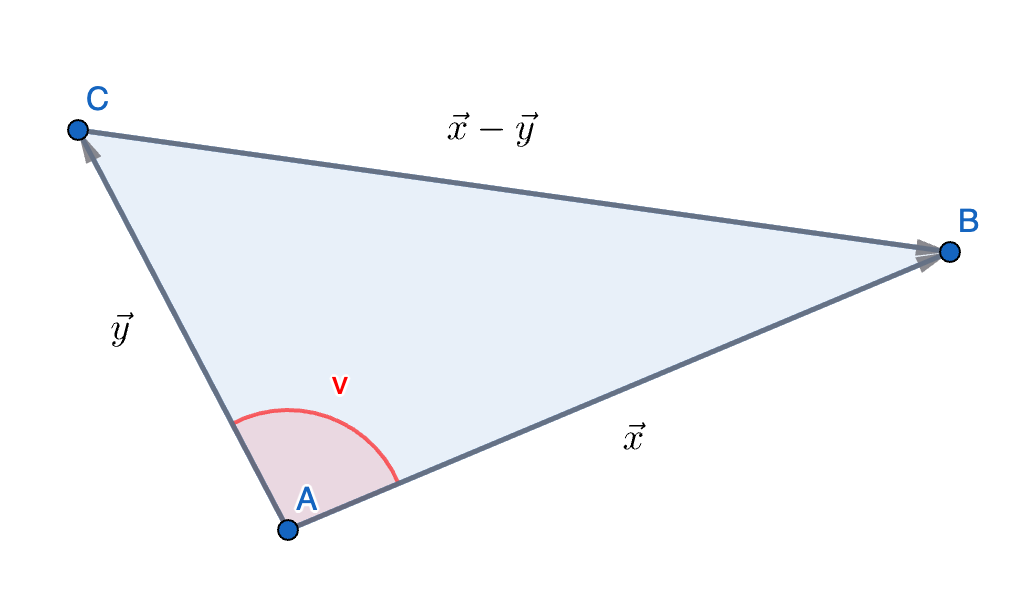
\includegraphics[scale=0.3]{./skitser/trekant_vektor_skitse.png}
    \label{fig:trekant_vektor}
    \caption{Vinkel udspændt af 2 vektorer.}
\end{figure}

Vha. af disse vektorer kan vi danne en trekant, hvori vi kan anvende cosinusrelationerne
til at lave et generelt udtryk for vinklen udspændt af 2 vektorer.
Her kan vi lave et udtryk for den lange side ved at anvende indskudsreglen:

\begin{align*}
    \vec{AB}+\vec{BC}&=\vec{AC}
    \\
    &\Downarrow
    \\
    \vec{BC}&=\vec{AC}-\vec{AB}
    \\
    &\Downarrow
    \\
    \vec{CB}&=-\vec{BC}=\vec{AB}-\vec{AC}
\end{align*}

Så den trejde side noteres $\vec{x}-\vec{y}$, og vi anvender cosinusrelationen, der siger, at i en trekant, så:

$$
    c^2=a^2+b^2-2ab \cdot \cos(v)
$$

Hvilket i vores tilfælde betyder:

$$
    |\vec{x}-\vec{y}|^2=|\vec{x}|^2+|\vec{y}|^2-2|\vec{x}||\vec{y}| \cdot \cos(v)
$$

Nu anvendes det, at $|\vec{x}|^2=\vec{x} \cdot \vec{x}$, det betyder for vores vektor:

$$
    |\vec{x}-\vec{y}|^2=(\vec{x}-\vec{y})\cdot (\vec{x}-\vec{y})
    =|\vec{x}|^2+|\vec{y}|^2-2 \cdot \vec{x}\cdot \vec{y}
$$

Det indsættes i ovenstående:

$$
\cancel{|\vec{x}|^2+|\vec{y}|^2-2} \cdot \vec{x}\cdot \vec{y}
=\cancel{|\vec{x}|^2+|\vec{y}|^2-2}|\vec{x}||\vec{y}| \cdot \cos(v)
$$

Hvor $\cos(v)$ isoleres:

$$
    \cos(v)=\frac{
        \vec{x} \cdot \vec{y}
    }{
        |\vec{x}||\vec{y}|
    }
$$
\end{proofw}
